
\section{Micro-Frontend Architecture}

Micro-frontends should bring the same advantages of microservices from the backend to the frontend. Instead of creating a large frontend monolith, a micro-frontend architecture contains many small applications. The advantage is that every micro-frontend can be developed and deployed by a separate team. \cite{book:2020:geers:micro-frontends-in-action} The difference between frontend-monoliths and micro-frontends can be seen in figure \ref{figure:state-of-the-art:ui-monolith-micro-frontend}.

\ifshowImages
\begin{figure}[H]
\centering
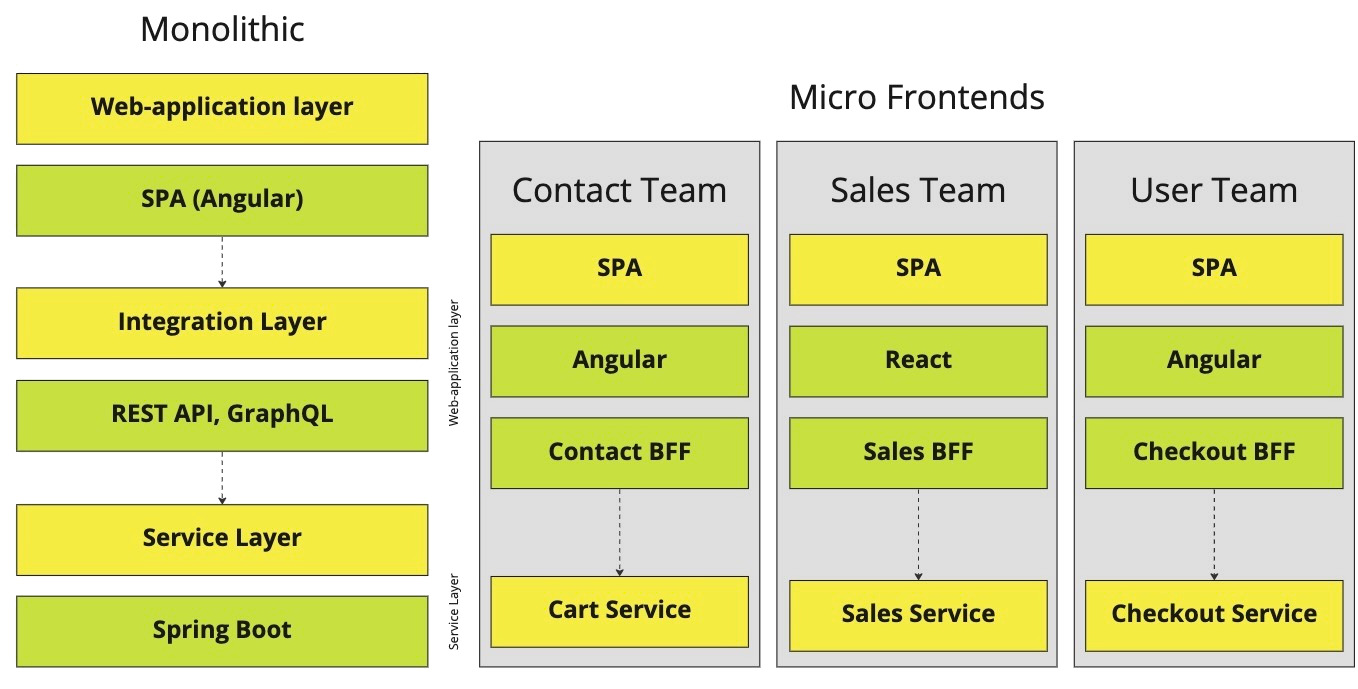
\includegraphics[width=0.8\linewidth]{images/ui-monolith-micro-frontends.jpeg}
\caption{A comparison between frontend-monoliths and micro-frontends.}\label{figure:state-of-the-art:ui-monolith-micro-frontend}
\end{figure}
\fi

Benefits gained from working with microservices on the backend are lost, when working with a monolithical frontend. With a monolithic frontend, the ability to deploy independently is lost. The entire frontend has to be deployed at once. Another problem is, that distinct operations are not really possible. If one part of the frontend is broken, there is a good chance that the entire frontend is broken. Another problem is the parallel development. The speed of development cannot be increased because it is very difficult to have multiple teams working on one frontend application. \cite{misc:2019:leitner:micro-frontends}

The term micro-frontend can be misleading, as can the term microservice. It has no meaning in terms of the size of the application. It can be a simple widget that only displays data, or a full-blown one-page application. Ideally, a micro frontend covers an area of the entire frontend application.


Micro-frontends try to apply the same principles from the microservice architecture to frontend development. Often times a microservice architecture with is developed by several teams has only one frontend application. Therefore, when adding new features a single team can be overwhelmed. Like a microservice architecture, a micro-frontend architecture focuses on developing many small frontend-applications, instead of developing a large software monolith. Each micro-frontend can be developed independently by another team. But a challenge is that the micro-frontend should appear as a single application to the user. Therefore, the different applications have to be integrated, which can be a challenge.

The term micro-frontend should not lead to false conclusions about the size of an application. The size of micro-frontends can vary. It can range from a simple login to a complex single-page application.

Building micro-frontends with the web allows different strategies of integrating the applications. Three different strategies exist to combine multiple micro-frontends into an app-shell. The client-side integration, the server-side integration and the combination of these two strategies and the combination of both strategies.

\subsection{Generic APIs vs Consumer Driven APIs}

The big decision in micro-frontend API development is to use either generic or consumer-oriented APIs. The difference is that generic APIs place great emphasis on reusability, while consumer-oriented APIs tailor the APIs to the customer.

\subsubsection{Generic APIs}

Generic APIs refer to APIs that are very general and can be used by different clients. However, this type of API has two major drawbacks. Over-fetching describes the problem of getting more data than is needed. Over-requesting describes the problem of needing multiple requests to get the data for a use case. Both problems are discussed in more detail in the next paragraphs. \cite{misc:2019:leitner:backend-for-frontends}

\paragraph{Over-Fetching}

For example, a contact service provides a contact-model that includes customer-number, first-name, second-name, uid-number and the address of the user, as seen in listing \ref{code:state-art:over-fetching}. However, one requirement of the application is to display only a contact's first and last name inside the header. Only two fields of the model are used, and the rest are unnecessarily queried. \cite{misc:2019:leitner:backend-for-frontends}

\ifshowListings
\begin{listing}[H]
\begin{minted}{typescript}
interface ContactModel {
  id: string;
  customerNumber: string;
  firstName: string;
  secondName: string;
  uidNumber: string;

  Address: {
    id: string;
    postalCode: string;
    location: string;
    Country: string;
  }
}
\end{minted}
\caption{Contact-Model that contains too much fields for the requirement.}\label{code:state-art:over-fetching}
\end{listing}
\fi

\paragraph{Over-Requesting}

Attempting to solve the problem of over-fetching by reducing the amount of data set that is returned leads directly to this problem. Listing \ref{code:state-art:over-requesting} shows the problem of over-requesting. If another requirement inside the application should display the address alongside the contact, two requests have to be performed every time. Afterwards, the two data sets have to be merged, which leads to high complexity on the client side. \cite{misc:2019:leitner:backend-for-frontends}

\ifshowListings
\begin{listing}[H]
\begin{minted}{typescript}
interface ContactModel {
  id: string;
  customerNumber: string;
  firstName: string;
  secondName: string;
  uidNumber: string;

  address_id: string;
}
\end{minted}
\caption{Contact-Model model that links the address-model with an id.}\label{code:state-art:over-requesting}
\end{listing}
\fi

\subsubsection{Consumer Driven APIs}

Consumer-driven APIs are the opposite of generic APIs. They follow the idea of providing the client with exactly the data it needs. Following the example above, the contact service would have an endpoint that returns only the first and last name as required for the request. These endpoints make communication with a client very simple and there is not the problem of over-fetching and over-requesting. However, creating an endpoint for each request creates an unmanageable set of endpoints. \cite{misc:2019:leitner:backend-for-frontends}

\subsubsection{Backend for Frontend}

\ifshowUnusedContent
TODO(FM): Too specific for the project report.
Every microservice provides its functionality to consumers with APIs. But it is not advisable that clients directly communicate with microservice APIs. Microservice offer fine-grained interfaces which were made especially for the communication between microservices. Therefore, the client usually has to make multiple requests to fetch the data needed for a view. ([7] S. Newman, Building microservices: designing fine-grained systems, First Edition. Beijing Sebastopol, CA: O’Reilly Media, 2015, (ISBN 978-1-4919-5035-7).

This leads to many requests, which is also known as over-requesting.

Another problem could be that a cluster of microservices use another form of communication. For example an asynchronous message-bus or another protocol like GRPC. There is the next problem. Clients usually communicate using synchronous communication, where microservices could use asynchronous communication. Without an adapter in between, the communication will not work properly. Even if the communication is possible, the client needs to know many details (IP-address) about the cluster of microservices. And the client might have to connect to multiple microservice to fetch the data needed to display one view. Therefore the client has to join the data in-memory. Changing the API of a microservice would have a ripple effect on the requests on the frontends, because they would have to be changed in many places.

[1] C. Richardson, Microservices patterns: with examples in Java. Shelter Island, New York: Manning Publications, 2019, (ISBN 978-1-61729-454-9).

To solve this problem the clients communicate with an API gateway or a more client centric backend-for-frontend service. Internally these services communicate with the microservice-cluster. An API gateway is a service that represents an abstraction of the microservice APIs and is an entry point to the microservice-cluster. The main task of a gateway is to forward tasks to the correct microservice. The even might implement functionalities like authorization and authentication or transform the protocol. Like transforming HTTP to GRPC. With API gateways it is also easier to split a microservice into two for example, without a ripple effect to change all clients as well.

But the problem with API gateways is the ownership. Multiple teams will add their functionality to the gateway and might come into conflict. The APIs are often not suited for the needs of clients and it has to be avoided that client logic is developed into the API gateway.

\fi

To solve these problems, the backend-for-frontend pattern is often used. This pattern provides each client with its own API, which specialized for the needs of the client. \cite{book:2018:richardson:microservices-patterns}

\ifshowImages
\begin{figure}[H]
\centering
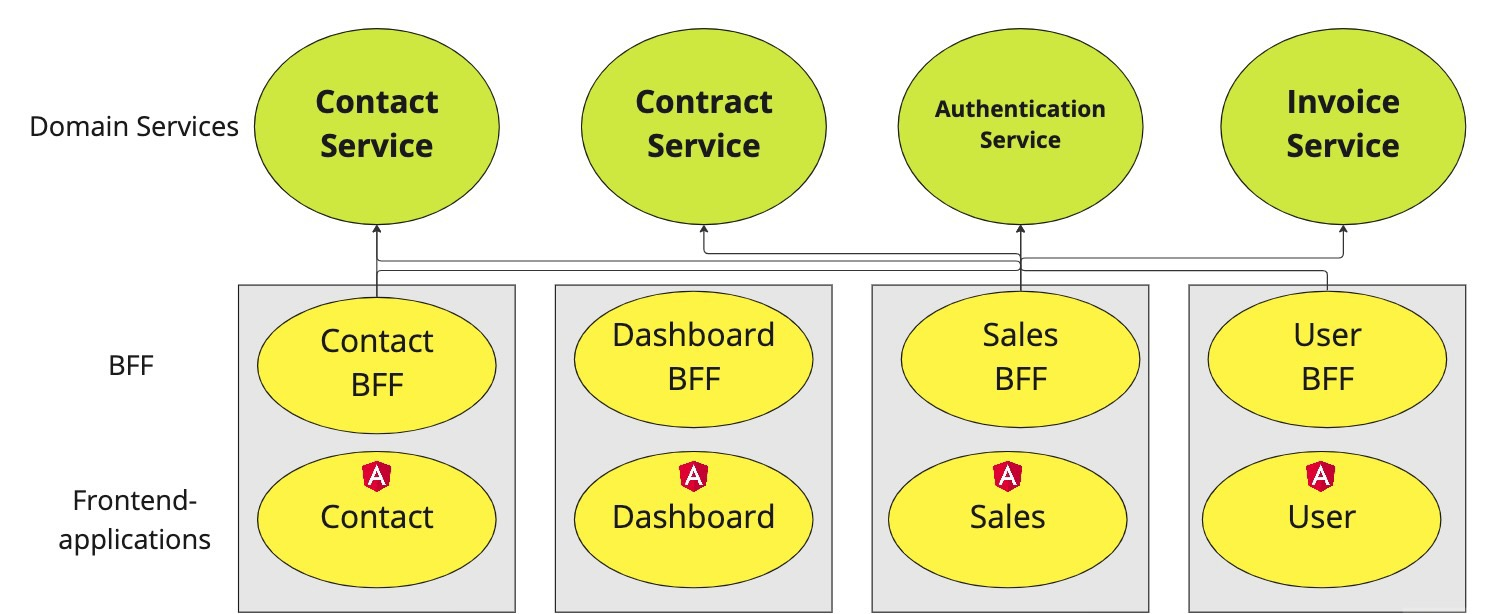
\includegraphics[width=0.8\linewidth]{images/ui-bff-architecture.jpeg}
\caption{Frontend architecture with the backend-for-frontend pattern.}\label{figure:state-of-the-art:ui-bff-architecture}
\end{figure}
\fi

Figure \ref{figure:state-of-the-art:ui-bff-architecture} shows an exemplary micro-frontend architecture using the backend-for-frontend pattern. Each frontend has a service that retrieves data only for that specific client. Because the backend-for-frontends function as gateway to the domain services, the domain services can stay very generic and be reused by different clients. Backend-for-frontends should implement only the presentation logic that puts the data into the form that the client needs. It should avoid storing state. \cite{misc:2019:leitner:backend-for-frontends}

With this architectural approach the backend-for-frontend and the frontend form a single deployment unit. If one application is changed, the other needs needs to adapt the changes. GraphQL is a perfect technology for implementing a backend-for-frontend, because it is specifically designed for implementing the presentation-layer.

\subsection{Characteristics}

Micro-frontends tend to follow the same characteristics as microservices.

\subsubsection{Autonomous}

Technically a micro-frontend is a completely independent and runnable application.
The integration of the micro-frontends happens only through the frontend. The different micro-frontends are composed withing an app-shell. The application shell is a separete application that is usually the entry-point for the user to interact with all micro-frontends. The app-shell also provides the layout of the page and defines where the micro-frontends are placed.

\subsubsection{Technology Agnostic}

Just as microservices architectures, micro-frontend architectures can be technology agnostic. The current frontend development landscape offers a lot of JavaScript frameworks to choose from.

\subsubsection{Independently Depoyable}

The autonomy of micro-frontends offer the possibility for independent deployments. A large monolithical micro-frontends is trickier to deploy. There is no need to have communication over multiple teams to deploy the application.


\subsubsection{Small and Easy to Maintain}



\subsubsection{Resilience}



\subsubsection{Resilience}



\subsection{Integration strategies}

\subsubsection{Server-Side Integration}
\subsubsection{Client-Side Integration}

\subsection{Communication}

\subsection{Backend-For-Frontend Pattern}
